\section{Vista de Desarrollo}

En la vista de desarrollo se distinguen dos proyectos principales, que se
corresponden con las carpetas del repositorio:

\begin{itemize}
  \item \textbf{Frontend} (\texttt{frontend/}): aplicación web en React que
        implementa la capa de presentación. Dentro de este proyecto se
        distinguen la UI (páginas y componentes) y los servicios de acceso a
        la API (hooks y funciones de \texttt{apiFetch}).
  \item \textbf{Backend} (\texttt{backend/}): aplicación Spring Boot que
        implementa las capas de aplicación, dominio e infraestructura. Se
        organizan los paquetes de controladores REST, servicios de
        negocio (Aplicación), entidades/agregados (Dominio) y componentes de
        infraestructura (repositorios, seguridad, envío de emails).
\end{itemize}

A nivel conceptual, estos proyectos respetan la separación en capas de
Presentación, Aplicación, Dominio e Infraestructura descrita en la
arquitectura de software.


\begin{figure}[H]
    \centering
    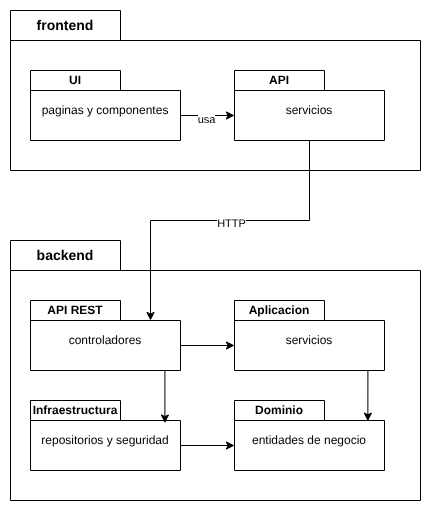
\includegraphics[width=0.6\textwidth]{img/diagrama_de_paquetes}
    \caption{Diagrama de Paquetes}
    \label{fig:dpkg}
\end{figure}

\begin{figure}[H]
    \centering
    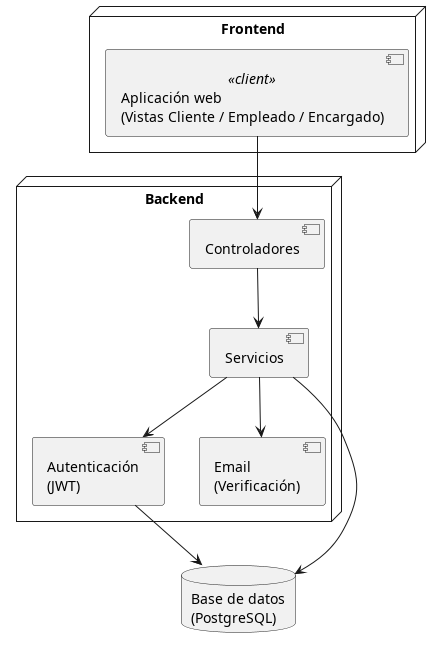
\includegraphics[width=0.6\textwidth]{img/diagrama_componentes}
    \caption{Diagrama de Componentes}
    \label{fig:dcmp}
\end{figure}

El diagrama de componentes muestra la interacción entre la aplicación web
frontend y los componentes principales del backend. El \textbf{Frontend} está
implementado como una SPA en React que ofrece distintas vistas para cliente,
empleado y encargado, y se comunica exclusivamente con la \textbf{API REST} del
backend mediante HTTP.

En el \textbf{Backend} se distinguen los controladores de la API, los
\textbf{servicios de negocio} (pedidos, catálogo, usuarios, descuentos), el
módulo de \textbf{autenticación} basado en JWT y tokens de refresh, y el
módulo de \textbf{email} utilizado para verificación de cuenta y recuperación
de contraseña. Todos estos componentes acceden a la \textbf{base de datos
PostgreSQL} a través de repositorios JPA, donde se persisten usuarios, pedidos,
productos, ingredientes, menús, descuentos y tokens.


\newpage